\documentclass[
    % -- opções da classe memoir --
    12pt,               % tamanho da fonte
    openright,          % capítulos começam em pág ímpar (insere página vazia caso preciso)
    oneside,
    a4paper,            % tamanho do papel. 
    % -- opções do pacote babel --
    english,            % idioma adicional para hifenização
    brazil              % o último idioma é o principal do documento
    ]{ifsp-spo-inf-ctds} % ajustar de acordo com o modelo desejado para o curso

% ---
% Informações de dados para CAPA e FOLHA DE ROSTO
% ---
\titulo{DESENHO DA APLICAÇÃO - PROJETO TURMA DE ELITE}

% Trabalho em Equipe
% ver também https://github.com/abntex/abntex2/wiki/FAQ#como-adicionar-mais-de-um-autor-ao-meu-projeto
\renewcommand{\imprimirautor}{
\begin{tabular}{lr}
     André Monteiro GOMES & SP3024059 \\
     Bianca Kaori HNG & SP3022455\\
     Gustavo Manoel SANTOS & SP3022391\\
     Luiz Henrique de Almeida e ALBUQUERQUE & SP3030199\\
     Natan da Fonseca LISBOA & SP3024784\\
     Patrícia Santos PASCHOAL & SP3022218
\end{tabular}
}


\disciplina{PI1A5 - Projeto Integrado I}

\preambulo{Trabalho apresentado ao Instituto Federal de Educação, Ciência e Tecnologia de São Paulo - Câmpus São Paulo - como parte dos requisitos para aprovação na disciplina Projeto Integrado I (PI1A5), do curso superior de Tecnologia em Análise e Desenvolvimento de Sistemas.}

\data{2021}

% Definir o que for necessário e comentar o que não for necessário
% Utilizar o Nome Completo, abntex tem orientador e coorientador
% então vão ser utilizados na definição de professor
\renewcommand{\orientadorname}{Professor:}
\orientador{DANIEL MARQUES GOMES DE MORAIS}


% ---


% informações do PDF
\makeatletter
\hypersetup{
        %pagebackref=true,
        pdftitle={\@title}, 
        pdfauthor={\@author},
        pdfsubject={\imprimirpreambulo},
        pdfcreator={LaTeX with abnTeX2 using IFSP model},
        pdfkeywords={abnt}{latex}{abntex}{abntex2}{IFSP}{\ifspprefixo}{trabalho acadêmico}, 
        colorlinks=true,            % false: boxed links; true: colored links
        linkcolor=blue,             % color of internal links
        citecolor=blue,             % color of links to bibliography
        filecolor=magenta,              % color of file links
        urlcolor=blue,
        bookmarksdepth=4
}
\makeatother
% --- 

% carregando aqui referencias quando utilizando BIBLATEX
\IfPackageLoaded{biblatex}{%
\addbibresource{referencias.bib}
\addbibresource{exemplos/abntex2-doc-abnt-6023.bib}
}{}

% ----
% Início do documento
% ----
\begin{document}

% ----------------------------------------------------------
% ELEMENTOS PRÉ-TEXTUAIS
% ----------------------------------------------------------
\pretextual

% ---
% Capa
% ---
\imprimircapa

% ---
% Folha de rosto
\imprimirfolhaderosto

% ---
% inserir lista de ilustrações
% ---
\pdfbookmark[0]{\listfigurename}{lof}
\listoffigures*
\cleardoublepage
% ---

% ---
% inserir lista de tabelas
% ---
\pdfbookmark[0]{\listtablename}{lot}
\listoftables*
\cleardoublepage
% ---

% ---
% inserir o sumario
% ---
\pdfbookmark[0]{\contentsname}{toc}
\tableofcontents*
% ---


% ----------------------------------------------------------
% ELEMENTOS TEXTUAIS
% ----------------------------------------------------------
\textual

\chapter[Introdução]{Introdução}
A participação dos alunos nas aulas e atividades escolares é essencial para a evolução do aprendizado. Porém, é possível observar que apenas a rotina de horas de aula combinada a um grande volume de atividades com poucas recompensas imediatas tendem a fazer com que os estudos se tornem maçantes para a maioria dos alunos, resultando na falta de motivação para desempenhar suas obrigações escolares.


No contexto educacional brasileiro, sabe-se que embora as escolas sejam obrigadas a seguir uma grade fixa de disciplinas e conteúdos de base, cada instituição possui sua maneira única de ofertá-lo aos seus alunos. Deste modo, surgiu o interesse de desenvolver uma solução que aplique conceitos de \textit{gamificação} na educação para motivar os alunos, mas que ao mesmo tempo seja flexível às necessidades dos diferentes clientes. 


Ademais, partindo de uma base de dados que será alimentada ao longo da utilização da aplicação, será possível desenvolver visões gerenciais que permitam aos diretores, pedagogos e professores acompanharem a evolução dos seus alunos, bem como diagnosticarem possíveis problemas e tomarem decisões para superá-los.

\section{Objetivos}
Este projeto visa desenvolver o sistema Turma de Elite, uma aplicação de gerenciamento de aprendizado que tem como objetivo integrar conceitos de \textit{gamificação} ao ensino, e deste modo se tornar uma ferramenta que busca auxiliar todo corpo docente e discente de uma instituição escolar.


Para o corpo docente, a ferramenta contará com funcionalidades que permitam acompanhar o desenvolvimento do aluno e modelar desafios, atividades e recompensas.


Para o corpo discente, a aplicação implementará funcionalidades que buscam promover o engajamento dos alunos nas aulas, acrescentando ao processo de realizar exercícios e avaliações, uma dinâmica semelhante aos jogos atuais onde ao completar um desafio, ganham-se recompensas, aumenta-se de nível e desbloqueia novos desafios.

\subsection{Objetivo Principal}
De modo geral, o projeto Turma de Elite tem a missão de promover um maior interesse dos alunos nos estudos por meio do aumento de fatores motivacionais na realização de tarefas, utilizando a \textit{gamificação} como elemento auxiliador nesse processo.

\subsection{Objetivos Secundários}
Tendo em vista a inserção tecnológica ocorrendo cada vez mais cedo na sociedade, coloca-se como objetivo secundário a maior disseminação da tecnologia no ambiente estudantil, de maneira benéfica.

\section{Justificativa}
Hoje em dia, já é possível encontrar plataformas educacionais online que aplicam o conceito de \textit{gamificação} para promover a aprendizagem do aluno. Entretanto, ao analisar as soluções existentes no mercado, percebe-se que a maioria possui uma deficiência em comum, não possuir código aberto. Este tipo de aplicação possui conteúdo engessado e é fortemente atrelado ao fabricante (\textit{\gls{vendor-lock-in}}). 


\section{Análise de concorrência}
\subsection{\textit{Khan Academy}}
Tomando uma plataforma como a \textit{Khan Academy}, que utiliza conceitos de \textit{gamificação} para a execução de atividades, nota-se que ela não utiliza o conceito de \textit{\glspl{tier}} para ranquear os alunos, por exemplo. Esse conceito compreende ao agrupamento de estudantes em ligas diferentes de acordo com o desempenho.

Outro diferencial em relação ao \textit{Khan Academy}, são as funcionalidades de customização de atividades, parametrização de turmas e conquistas que permitem que a Turma de Elite se adapte não só a diferentes escolas como também às categorias de ensino remoto e à distância.

\subsection{\textit{Academy LMS}}
Essa outra solução, por sua vez, já possui suporte para múltiplas visões de usuário.
Entretanto, como ela não possui código aberto, uma forma de obtenção de lucro encontrada foi a cobrança por meio de uma assinatura.

\subsection{\textit{Axonify}}
Esse sistema de gestão de aprendizagem possui algumas funcionalidades interessantes no que diz respeito à implementação de \textit{gamificação}, como pontos, conquistas, medalhas e \textit{\glspl{ranking}}. Entretanto, tal solução também não possui código ou visão para um administrador. 

\subsection{\textit{Matrix LMS}}
Dentre as soluções verificadas, essa se mostrou a solução mais completa, uma vez que possui todas as visões de usuário que a Turma de Elite pretende implementar (aluno, professor e gestor). Entretanto, uma grande desvantagem dela é o custo, uma vez que, além de uma assinatura ser cobrada para continuar utilizando a plataforma, os materiais oferecidos também são pagos.  

\subsection{\textit{Talent LMS}}
Ao analisar o \textit{Talent \ac{lms}}, pode-se constatar algumas ausências importantes para um sistema de aprendizagem gamificado, como a premiação com medalhas. Apesar disso, esse sistema compensa tal ausência com a implementação de pontos e níveis.


\subsection{\textit{Moodle} + \textit{Level Up}!}
Uma outra opção possível para gamificar o ensino é a incorporação de um \textit{\gls{plugin}} que ofereça ferramentas de gamificação a um sistema de \textit{\ac{lms}} já consolidado no mercado. Ao analisar as funcionalidades de um \textit{\gls{plugin}} de \textit{gamificação} \textit{\gls{open-source}} chamado \textit{"Level Up!"}, nota-se que ele não contempla algumas funcionalidades para sua utilização no contexto de gestão de uma instituição de ensino, como a visão de gestor, por exemplo.
A Tabela 1 contém a comparação sintetizada de todos os sistemas analisados.

% \ABNTEXfontereduzida
\begin{table}[htb]
\label{tabela1}
\centering
\caption{Análise comparativa entre as plataformas de gestão de aprendizado}
\begin{tabular}{|m{2.3cm}|m{1.8cm}|m{1.8cm}|m{1.5cm}|m{1.5cm}|m{1.2cm}|m{1.5cm}|m{1.3cm}|m{1.8cm}}
\hline
{\thead{}} & \thead{Khan\\ Academy} & \thead{Academy\\ LMS} & \thead{Axonify} & \thead{Matrix \\LMS} & 
\thead{Talent \\ LMS} & 
\thead{Moodle \\+ Level\\ Up!} &
\thead{Turma\\ de \\elite} \\ \hline
    Código aberto               &   &   &   &   &   & X & X               \\ \hline
    Customização de atividades  &   & X & X & X & X & X & X               \\\hline
    Medalhas                    & X & X & X & X & X & X & X               \\ \hline
    Tiers / ligas               &   &   &   &   &   &   & X               \\ \hline
    Leaderboards                & X & X & X & X & X & X & X               \\ \hline
    Visão do Gestor             &   &   &   & X &   &   & X \\ \hline   
\end{tabular}
\fonte{Os autores}
\end{table}
\chapter{Revisão da Literatura}

\section{\textit{Learning Management System (LMS)}}
Os \textit{\ac{lms}} – plataformas de apoio à aprendizagem - surgiram para dar apoio à formação a distância online. As plataformas facilitam a disponibilização de recursos em diferentes formatos como texto, vídeo e áudio, apontadores para sites, avisos, interação professor-alunos através de ferramentas de comunicação, ferramentas de apoio à aprendizagem colaborativa e registro das atividades realizadas pelos alunos \cite{rentabilizacao-ens-basico-e-secundario:2007}.


\section{\textit{Gamificação}}
A \textit{gamificação} é uma técnica que envolve dinâmicas, mecanismos e elementos dos \textit{videogames} e os aplica em contextos da vida real. O principal objetivo é engajar as pessoas para que mudem alguns comportamentos, com o propósito de alcançar resultados relacionados a objetivos específicos.


A \textit{gamificação} surge justamente para auxiliar nessa demanda. Em situações em que o engajamento é precário, é possível estabelecer um estímulo extra em contextos que nada têm a ver com jogos, como ambientes corporativos e educacionais.
\cite{gamificacao-corporativa:2017}


Desse modo, pode-se afirmar que a \textit{gamificação} é um processo dedicado ao engajamento de pessoas para que elas produzam mais, independentemente do setor em que estejam inseridas.
\cite{gamificacao-corporativa:2017}


\section{Recompensa}
A recompensa se refere a um prêmio ou retribuição por algo \cite{dicio-recompensa:2009}


Todos gostam de se sentir valorizados por aquilo que produzem. Assim é importante que os gestores se lembrem de implementar alguns mecanismos de recompensas que motivem os colaboradores. \cite{gamificacao-corporativa:2017}


Em uma pesquisa realizada pela \textit{\gls{aberdeen}}, constatou-se que mais da metade dos entrevistados associam a motivação com o reconhecimento por performance. A Figura 1 mostra os fatores motivacionais:

\begin{figure}[htb]
    \centering
	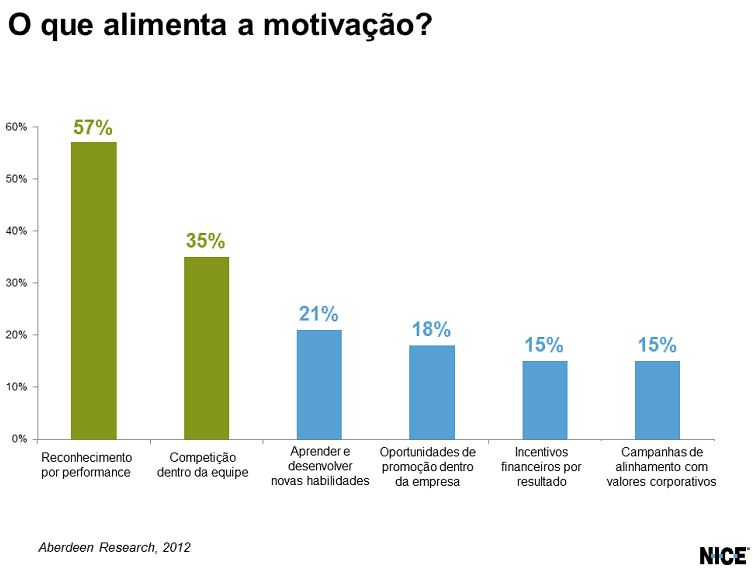
\includegraphics[width=16cm]{imagens/recompensa.jpg}
	\caption{O que alimenta a motivação?}
	\fonte{\cite{grafico-motivacao:2012}}
\end{figure}
\FloatBarrier

\section{Tecnologias}
\subsection{Java}
Java é uma linguagem de programação e plataforma computacional lançada pela primeira vez pela \gls{sun-microsystems} em 1995.


Para criar \textit{applets} e aplicações Java, são necessárias ferramentas de desenvolvimento como o {\ac{jdk}}. O {\ac{jdk}} inclui o \gls{java-runtime-environment}, o \gls{compilador-java} e as \gls{api-java}. É fácil começar a desenvolver programas em Java, tanto para os novos programadores quanto para os experientes \cite{java:2016}.


No projeto Turma de Elite, a linguagem de programação Java será utilizada no \textit{back-end}, apoiado pelo \textit{\gls{framework}} Spring e seus componentes.


\subsection{Spring}
O Spring Framework fornece um modelo abrangente de programação e configuração para aplicativos empresariais modernos baseados em Java - em qualquer tipo de plataforma de implantação.


Um elemento-chave do Spring é o suporte de infraestrutura no nível do aplicativo: o Spring se concentra na "canalização" dos aplicativos corporativos para que as equipes possam se concentrar na lógica de negócios no nível do aplicativo, sem vínculos desnecessários com ambientes de implementação específicos \cite{spring:2021}.

\subsection {Angular}
Angular é uma plataforma de desenvolvimento, construída em 
TypeScript, que inclui:
\begin{itemize}
\item Uma estrutura baseada em componentes para a construção de aplicativos da \textit{\gls{web}} escaláveis;
\item Uma coleção de bibliotecas bem integradas que cobrem uma ampla variedade de recursos, incluindo roteamento, gerenciamento de formulários, e comunicação cliente-servidor;
\item Um conjunto de ferramentas de desenvolvedor capaz de ajudar a desenvolver, construir, testar e atualizar o código \cite{angular:2021}.
\end{itemize}

Será utilizado o Angular como \textit{\gls{framework}} para o \textit{\gls{front-end}} do projeto.

\subsection{MySQL}
Para armazenamento de dados foi escolhido o MySQL. Esse é o banco de dados de código aberto mais popular do mundo. Com seu desempenho comprovado, confiabilidade e facilidade de uso, o MySQL se tornou a principal escolha de banco de dados para aplicativos baseados na web, usados por propriedades da \textit{\gls{web}} de alto perfil, incluindo Facebook, Twitter, YouTube, Yahoo! dentre outros \cite{mysql:2021}.

\subsection{GitHub}
O GitHub oferece um serviço de hospedagem de repositório \gls{git} baseado em nuvem, tornando assim muito mais fácil para que indivíduos e equipes usem o \gls{git} para controle de versão e colaboração.


A interface do GitHub é amigável o suficiente para que até programadores novatos possam utilizar o \gls{git} com facilidade. Sem o GitHub, seria necessário um pouco mais de conhecimento técnico e o uso da linha de comando para o uso do \gls{git} \cite{github:2021}.

\subsection{SVN}
Subversion (\ac{svn}) é um sistema de controle de versão de código aberto. Fundado em 2000 pela CollabNet, \ac{inc}, o projeto e o \textit{\gls{software}} Subversion tiveram um sucesso incrível na última década. O Subversion tem desfrutado e continua a ter ampla adoção tanto na arena do código aberto quanto no mundo corporativo \cite{svn:2021}.


Durante o desenvolvimento, serão utilizados o GitHub e o \ac{svn} para o versionamento de código.

\subsection{Heroku}
Heroku é uma plataforma em nuvem que permite às empresas criar, entregar, monitorar e dimensionar aplicativos, sendo a maneira mais rápida de ir da ideia à \ac{url}.


A plataforma foca incansavelmente em aplicativos e na experiência do desenvolvedor em torno de aplicativos. O Heroku permite que empresas de todos os tamanhos adotem o valor dos aplicativos \cite{heroku:2021}.

\subsection{Travis CI}
Travis \ac{ci} é um serviço de integração onde é possível sincrinizar projetos de código aberto hospedados no GitHub \cite{travis:2021}.

\subsection{Firebase Hosting}
O Firebase Hosting é um recurso de hospedagem de conteúdo da \textit{\gls{web}} de nível de produção para desenvolvedores, sendo possível facilmente implantar apps da \textit{web} de forma rápida e exibir conteúdo estático e dinâmico a uma rede de distribuição de conteúdo (\ac{cdn}) global \cite{hosting:2020}.


O \textit{\gls{back-end}} da aplicação será hospedado no Heroku, utilizando como plataformade \ac{ci}, o Travis. O \textit{\gls{front-end}} da aplicação será hospedado com o serviço Firebase Hosting, do Google.


\subsection{Firebase Authentication}
A maioria dos \textit{\glspl{app}} precisa reconhecer a identidade do usuário. Ter essa informação permite que um \textit{\gls{app}} salve os dados do usuário na nuvem com segurança e forneça a mesma experiência personalizada em todos os dispositivos do usuário \cite{authentication:2020}.


O Firebase Authentication fornece serviços de \textit{\gls{back-end}}, \ac{sdk} fáceis de usar e bibliotecas de \ac{iu} prontas para autenticar usuários no seu aplicativo. Ele oferece suporte à autenticação usando senhas, números de telefone, provedores de identidade federados conhecidos, como Google, Facebook e Twitter, entre outros.


Para dar suporte à autenticação de usuário no sistema, será utilizado o Firebase Authentication.

\chapter{Gerenciamento do Projeto}
Este capítulo visa definir a parte de gestão de projeto, incluindo a metodologia adotada, a organização da equipe e a gestão do tempo.

\section{Metodologia de Gestão}
A metodologia de gerenciamento de projeto adotada é baseada no Scrum.

O Scrum é um \textit{\gls{framework}} para gestão de projetos que tem como principais objetivos agilizar o processo de desenvolvimento do \textit{\gls{software}} e responder rapidamente às mudanças. Ela é composta por cerimônias e tem como um dos pilares as \textit{\glspl{sprint}}, ou seja, um conjunto de atividades para um determinado tempo. 


As atividades de uma \textit{\gls{sprint}} serão planejadas em uma \textit{Sprint Planning}, que é a primeira cerimônia e tem como principal objetivo a definição das entregas para o final da \textit{\gls{sprint}}. Nessa cerimônia, baseando-se nas histórias priorizadas no \textit{Product Backlog}, será criado o \textit{Sprint Backlog} em um arquivo em Excel, que contém as atividades e suas principais informações, como o responsável, o status, podendo ser \textit{To Do} (a fazer), \textit{Doing} (fazendo) e \textit{Done} (feito), e a data de conclusão. 


Após o planejamento da \textit{\gls{sprint}}, a execução das atividades será iniciada. A \textit{\gls{daily}} será feita através do aplicativo \textit{\gls{notion}}, no qual cada um colocará as atividades feitas no dia, os próximos passos e os impedimentos, caso houver. Além disso, reuniões de acompanhamento serão feitas para ver o andamento do projeto e alinhamento das expectativas da \textit{\gls{sprint}}. Desse modo, esses \textit{\glspl{checkpoint}} semanais acontecerão nas terças-feiras às 19:30 ao longo da sprint. 

No último dia da \textit{\gls{sprint}}, às 19h30, será feita uma reunião para revisão das entregas, a chamada \textit{Sprint Review}, na qual será identificado o que foi entregue com sucesso, o que não foi concluído e também possíveis mudanças no \textit{\gls{product-backlog}}. 


Após a \textit{Sprint Review}, será feita uma reunião de retrospectiva, a \textit{Sprint Retrospective}, para avaliar o desempenho da equipe, o andamento do projeto e possíveis melhorias para a próxima \textit{\gls{sprint}}. A \textit{Sprint Planning} da \textit{\gls{sprint}} seguinte será realizado logo após a \textit{Sprint Review} da anterior.


Todas as reuniões acontecerão através do \textit{Google Meet}.
Para eventuais dúvidas, alinhamentos e possíveis urgências será utilizado o \textit{WhatsApp} e, se necessário, reuniões no \textit{Google Meet}. 


\section{Organização da Equipe}
As atividades foram divididas entre os integrantes da equipe segundo as habilidades e interesses de cada um, levando-se em consideração também o nível de dificuldade de cada frente.


Desse modo, o André será o \textit{\gls{tech-lead}} da equipe e focará na frente de desenvolvimento do sistema, portanto a parte de preparação do ambiente, desenvolvimento \textit{\gls{back-end}} e \textit{\gls{front-end}} serão as suas principais atividades, mas também atuará na elaboração de documentação, na fase inicial do projeto, e como suporte, ao longo dele.


A Bianca será a gerente de projetos e \textit{\gls{scrum-master}} da equipe, sendo a responsável por organizar a equipe e por garantir as entregas do projeto. Será responsável também pela postagem no blog semanalmente e auxiliará na elaboração da documentação e na criação dos vídeos. E poderá auxiliar nas outras frentes conforme houver necessidade.


O Luiz fará parte do time de desenvolvimento e auxiliará no desenvolvimento \textit{\gls{back-end}}, sobretudo na parte de testes, e \textit{\gls{front-end}}, na estilização das telas, mas também atuará, principalmente, na frente da documentação. Ele auxiliará também na parte dos vídeos e poderá desempenhar outras funções conforme houver necessidade.


O Natan também fará parte do time de desenvolvimento e auxiliará no desenvolvimento do \textit{\gls{back-end}}, na parte de testes e no desenvolvimento da aplicação em si, mas também focará na documentação. Será o principal responsável pela criação, edição e postagem dos vídeos e também poderá atuar nas outras frentes conforme houver necessidade.


A Patrícia será a \textit{\gls{product-owner}} e terá como principal foco a documentação, principalmente a elicitação de requisitos e definição do escopo. Ela cuidará também da frente dos Dados da aplicação e auxiliará no \textit{\gls{front-end}}, sobretudo na parte de protótipos de telas. E poderá auxiliar nas outras frentes conforme houver necessidade.


\section{Gestão de Tempo}

Baseando-se no Scrum, a gestão do tempo será feita pelas \textit{\glspl{sprint}}. Cada \textit{\gls{sprint}} terá a duração de duas semanas e, no total, serão quinze \textit{\glspl{sprint}}, com previsão de datas de início e de fim conforme descrito na Tabela 2. 


\ABNTEXfontereduzida
\begin{table}[htb]
\centering
\caption{Data de início e data fim de cada \textit{sprint}}
\begin{tabular}{|c|c|c|}
   \hline
   \thead{Sprint} & \thead{Data Início}  & \thead{Data Fim}   \\\hline
    1 & 10/05/21 & 25/05/21 \\\hline
    2 & 25/05/21 & 08/06/21 \\\hline
    3 & 08/06/21 & 22/06/21 \\\hline
    4 & 22/06/21 & 06/07/21 \\\hline
    5 & 06/07/21 & 20/07/21 \\\hline
    6 & 20/07/21 & 03/08/21 \\\hline
    7 & 03/08/21 & 17/08/21 \\\hline
    8 & 17/08/21 & 31/08/21 \\\hline
    9 & 31/08/21 & 14/09/21 \\\hline
    10 & 14/09/21 & 28/09/21 \\\hline
    11 & 28/09/21 & 12/10/21 \\\hline
    12 & 12/10/21 & 26/10/21 \\\hline
    13 & 26/10/21 & 09/11/21 \\\hline
    14 & 09/11/21 & 23/11/21 \\\hline
    15 & 23/11/21 & 14/12/21 \\\hline
\end{tabular}
\fonte{Os autores}
\end{table}
\FloatBarrier


As atividades priorizadas para cada \textit{\gls{sprint}} serão baseadas no cronograma da disciplina e serão agrupadas visando a sua finalização até o final da \textit{\gls{sprint}}, mas dependendo da dificuldade da atividade, ela poderá ser iniciada em uma \textit{\gls{sprint}} e terminar em outra.
\chapter{Arquitetura de solução}
\section{Arquitetura da solução apresentada}
A arquitetura da solução proposta será baseada, de uma forma geral, na arquitetura \ac{mvc}. Este modelo é apresentado em camadas que separam a apresentação e a interação de dados no sistema. É estruturado em três componentes: O modelo é responsável pelo gerenciamento dos dados, a visão que gerencia a apresentação dos dados e o controlador, responsável por intermediar a comunicação entre os eventos gerados pelo usuário na interface e o modelo \cite{engenharia-de-software:2018}

O diagrama apresentado pela Figura 2, mostra o modelo arquitetural adotado.

\begin{figure}[htb]
    \centering
	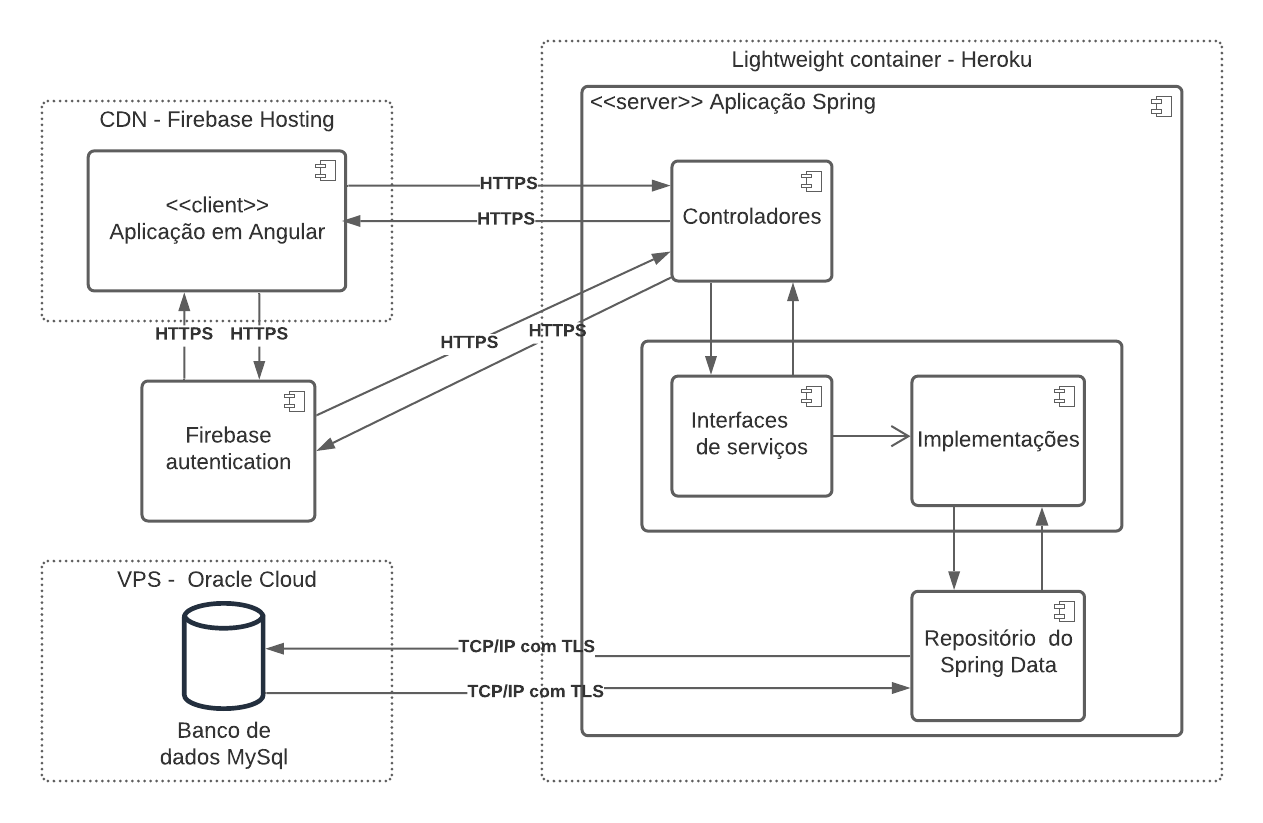
\includegraphics[width=16cm]{imagens/figura2.png}
	\caption{\label{fig_logo} Arquitetura da solução}
	\fonte{Os autores}
\end{figure}
 
 
De modo a desenvolver uma aplicação que busca garantir uma boa usabilidade, e capaz de aproveitar os recursos disponíveis da melhor forma, para a interface do usuário (\textit{\gls{front-end}}) será adotado o modelo arquitetural Single Page Aplication (\ac{spa}). 


Neste modelo, a maioria dos recursos necessários é carregada na inicialização da aplicação, fazendo com que não seja necessário recarregar a página durante o uso. A única mudança que ocorre é a dos dados, que são trafegados entre o servidor e o cliente.


Conforme o diagrama apresentado pela Figura 2, as camadas que compões a solução utilizam as seguintes infraestruturas para hospedagem:
\begin{itemize}
\item \ac{cdn} (Firebase Hosting): infraestrutura responsável por hospedar a aplicação em Angular, da camada de visão. Um serviço de hospedagem, que tem como base o armazenamento em \ac{ssd} e uma \ac{cdn}, totalmente gerenciado para conteúdo estático e dinâmico.
\item  Lightweight container (Heroku): infraestrutura responsável por hospedar a aplicação Spring, da camada controladora. A tecnologia utilizada pelo Heroku, utiliza o conceito de \textit{\gls{container}} que empacota o código e as dependências do aplicativo abstraindo o gerenciamento do \textit{\gls{hardware}}, levando a simplificação do desenvolvimento e o aumento da produtividade.
\item \ac{vps} (Oracle Cloud): infraestrutura responsável por hospedar o banco de dados da aplicação. Esta infraestrutura oferece um alto poder de computação e segurança.
\end{itemize}
Para a autenticação da aplicação, será utilizado o Firebase Authentication. Essa tecnologia oferece o serviços, \ac{sdk} e bibliotecas prontas para autenticar usuários. Sabe-se que a utilização deste serviço trará a aplicação a característica de \textit{\gls{vendor-lock-in}}, isto é, dependente de uma tecnologia terceira.  Porém, as vantagens ofertadas de segurança e a facilidade de implementação levaram a sua adoção ao projeto. 

Ademais, para minimizar os impactos negativos da utilização de uma tecnologia terceira, o Firebase Authentication será implantado seguindo o padrão de projeto \textit{Adapter}. Deste modo, diante da necessidade, a tecnologia poderá ser facilmente substituída por outra ou até mesmo por uma proprietária.


\section{Arquitetura de comunicação entre as camadas}
A comunicação entre a camada de visão e a camada controladora, será realizada via protocolo \ac{https}. Este protocolo acrescenta uma camada a mais de segurança à aplicação, uma vez que utiliza a criptografia na transferência de recursos.


Já a comunicação entre os controladores e banco de dados, será realizada via TCP/IP acrescido do protocolo \ac{tls} que aumenta a segurança através de criptografia, a interoperabilidade, a extensibilidade e a eficiência;


\section{Necessidade de escalabilidade}
A escalabilidade da aplicação estará intimamente ligada à infraestrutura adotada. Como aplicação será hospedada utilizando serviços de nuvem como Heroku e Firebase Hosting, categorizados como \ac{paas}. Os detalhes de infraestrutura são abstraídos facilitando a manutenção, extensão e escalabilidade além de oferecer baixo custo inicial. 

Como a princípio a aplicação será ofertada a um número pequeno de usuários, o plano  gratuito já será suficiente para comportar o número de acessos. E assim, conforme a necessidade será possível escalar a aplicação mediante a contratação de pacotes com mais recursos.
\chapter {Segurança}
\section {Critérios de Segurança, Privacidade e Legislação}
Todos os dados e informações pessoais inseridas para cadastramento serão mantidos em sigilo pelo sistema, como previsto na Lei Geral de Proteção de Dados, que regulamenta e controla processos relacionados a dados pessoais, visando proteger a liberdade e privacidade dos usuários.


Para realizar tal proteção de dados, seguiremos alguns pontos vitais para que os dados estejam guardados da maneira mais segura possível, seguindo os \textbf{Pilares da Segurança da Informação}.
\section {Pilares}
\begin{itemize}
\item \textbf{Confidencialidade}: garante que as informações estarão acessíveis somente para pessoas autorizadas, exigindo autenticação para restringir acessos;
\item \textbf{Integridade}: mantém a origem das informações conforme foram armazenadas, sem alterá-las;
\item \textbf{Disponibilidade}: faz com que os dados estejam disponíveis para usuários autorizados a qualquer momento que for necessário;
\item \textbf{Autenticidade}: identifica e registra usuários que estejam enviando ou modificando informações, para que essa ação seja documentada;
\end{itemize}
\chapter{Manutenibilidade da aplicação}

\section{Testes automatizados e análise estática}


Como o \textit{\gls{back-end}} da aplicação será desenvolvido em Java, a ferramenta adotada para automatização de testes é o JUnit. O JUnit é um \textit{\gls{framework}} de código aberto que auxilia o desenvolvimento de testes que verificam o funcionamento das classes e seus métodos. Ademais, a utilização do JUnit permite que toda estrutura de testes criada, seja executada a cada atualização da aplicação  de modo a garantir sua estabilidade e integridade.


No \textit{\gls{front-end}} serão adotados os \textit{glspl{framework}} de testes para Angular; Jasmine e Karma. Com o Jasmine, os testes poderão ser escritos de maneira independente do navegador e de bibliotecas para seu funcionamento. O Karma será utilizado para automatizar testes e executá-los para diversos navegadores a partir de um único comando. Com o Karma, além de testes unitários, também é possível realizar testes de integração e \ac{e2e}.


Todas as ferramentas escolhidas serão configuradas com servidores de integração contínua (\ac{ci}) de modo a manter o projeto livre de erros e inconsistências.


A análise estática do código no \textit{\gls{back-end}} será realizada pela ferramenta \textit{\gls{deep-source}}. A ferramenta possui integração nativa com o GitHub que permite revisão do código durante todo processo de desenvolvimento do projeto, além de permitir rastrear métricas de código como cobertura de testes e de documentação. No \textit{front-end} a análise será realizada pelo próprio \textit{\gls{eslint-schematics}} do Angular.


\section{Sistemas de \textit{log}}
Gerenciar os \textit{\glspl{log}} da aplicação é essencial para manter sua integridade. Com os \textit{\glspl{log}} é possível analisar as operações internas da aplicação, permitindo uma maior rastreabilidade que fornecem informações necessárias para resolução de possíveis problemas na aplicação.


O sistema de \textit{\gls{log}} \gls{journalctl} foi adotado para o MySql. Ele será responsável por registrar os logs de entrada e saída da \textit{console}. 
Para o \textit{back-end} será utilizado o \ac{slf4j} com saída para o Heroku.  Nos logs do Heroku será possível visualizar: 
\begin{itemize}
\item Logs do aplicativo através do comando “--source app”;
\item Registros do sistema através do comando “--source heroku”;
\item Logs de \textit{\ac{api}} através do comando “--source app --dyno api”.
\end{itemize}


No \textit{front-end} será utilizado o \textit{\gls{cloud-logging}} do \textit{Firebase Hosting} com o padrão de objeto console recomendado para desenvolvimento Web. Com essa ferramenta é possível visualizar:
\begin{itemize}
\item Logs com nível de registro INFO com os comandos "console.log()" e console.info();
\item Logs com nível de registro ERROS com os comandos "console.warn()" e "console.error()";
\item Mensagens internas com nível de registro DEBUG.
\end{itemize}
\section{Integração contínua}
O processo de integração contínua se inicia a partir da liberação de uma nova funcionalidade; através do \textit{\gls{pull-request}}, os desenvolvedores serão notificados da necessidade de realizar o \textit{\gls{merge}}; neste momento, a equipe deverá se reunir para realizar a revisão do código. Esta revisão inclui a análise dos resultados dos testes configurados, caso todas as métricas de código seja atingida, é realizado um \textit{\gls{merge}} com a \textit{\gls{branch-develop}}. 


Quando houver a necessidade de realizar o \textit{\gls{deploy}} da aplicação, basta apenas realizar o \textit{merge} com a branch release. Nela, a \textit{\gls{build}} da aplicação será feita de forma automática, e a aplicação estará atualizada no servidor. 


A ferramenta escolhida para automatizar o processo de \textit{\gls{build}} de aplicação e  apoiar a equipe no processo de \ac{ci} e \ac{cd} é o Travis CI.


\section{\textit{Coding Convention}}
Para a solução será adotada serão adotadas as diretrizes padrões da própria linguagem de programação descritas nas seguintes documentações:

\begin{itemize}
\item Back-end: sintaxe da linguagem JAVA  apresentados descritos na documentação Java Code Conventions \cite{javacodeconvention:1997}.
\item Front-End: sintaxe descrita no guia de estilo de codificação na documentação do angular. \cite{angularstyleguide:2021} 
\end{itemize}


Utilizar as convenções de códigos padrões é de extrema importância para a manutenibilidade da aplicação, pois tornam o código mais legível e facilitam o entendimento de desenvolvedores que futuramente poderão se tornar responsáveis por manter o software.



\section{\textit{Design Pattern}}
Para a aplicação serão adotados os seguintes padrões de projeto:
\begin{itemize}
\item  Observer: este padrão de projeto do tipo comportamental define um mecanismo de assinatura que notifica os objetos observadores a respeito dos eventos que acontecem a um objeto observado. 
Este padrão é amplamente utilizado pelo no Angular, \textit{\gls{framework}} adotado no desenvolvimento da do \textit{\gls{front-end}} da aplicação. Nele, os observáveis apoiam a transmissão de mensagens entre os componentes da aplicação, sejam elas mensagens literais, mensagens ou eventos.
\item Adapter: este padrão de projeto do tipo estrutural, é utilizado quando existe a necessidade de unir duas interfaces independentes ou incompatíveis. Na aplicação ele será utilizado na implementação do Firebase Authentication, de modo a garantir uma substituição por outro serviço de autenticação de modo fácil diante de uma futura necessidade.
\end{itemize}

\chapter{Escopo do Projeto}
A proposta de projeto é uma aplicação \textit{web} voltada para auxiliar no acompanhamento da evolução no rendimento dos alunos nas atividades escolares.

\section{Histórias de Usuário}
Para o projeto, foram escolhidas as histórias de usuário para estabelecer as necessidades do sistema. 

\subsection{Cadastros}
Eu, como administrador, quero criar outro administrador, para que alguém possa me ajudar nas tarefas administrativas do sistema

Eu, como administrador, gostaria de cadastrar escolas para meus clientes.

Eu, como administrador, gostaria que, ao criar uma escola, fosse enviado um e-mail para o gestor com uma página para que ele complemente as informações da escola e do seu usuário.

Eu, como administrador, quero visualizar um resumo do uso do sistema, para que eu possa tomar decisões com base no uso.

\subsection{Acessos e Logins}

Eu, como usuário do sistema, gostaria de poder definir a minha senha durante o primeiro acesso a aplicação para garantir a segurança do acesso.

Eu, como usuário do sistema, gostaria de fazer o login na aplicação para garantir a privacidade dos meus dados.

Eu, como usuário do sistema, gostaria de poder recuperar minha senha.

Eu, como administrador, quero revogar os acessos de outro administrador, para caso ele seja demitido da empresa.

Eu, como administrador, quero revogar os acessos de um gestor e sua escola, para caso eles criem conteúdos inadequados.

Eu, como administrador, quero desativar a escola, para suspender o uso de seus usuários quando os mesmos estiverem em débito com a empresa.

\subsection{Parametrização de turmas}

Eu, como gestor, gostaria de cadastrar uma nova turma para os alunos do próximo ano letivo.

Eu, como gestor, gostaria de dar o cargo de professor a um novo usuário caso um novo professor seja contratado.

Eu, como gestor, gostaria de atribuir professores e alunos as suas devidas disciplinas para facilitar a interação entre ambos os lados.

Eu, como gestor, gostaria de atribuir dois professores em uma mesma disciplina para uma turma de alunos que pode ser dividida.

\subsection{Painel de turmas}
Eu, como gestor, gostaria de visualizar todas as turmas e disciplinas cadastradas para uma melhor administração das mesmas.

Eu como professor, gostaria de visualizar as turmas atribuídas a mim para postar meus conteúdos por turma.

\subsection{Atividades}
Eu, como professor, gostaria de cadastrar atividades no sistema para que meus alunos façam.

Eu, como professor, gostaria de marcar se uma atividade é avaliativa ou não e se é entregável ou não para poder atribuir melhor as conquistas.

Eu, como aluno, gostaria de ter fácil acesso às minhas atividades, para não perder tempo procurando-as.

Eu, como aluno, gostaria de poder visualizar as minhas atividades ordenadas por data de vencimento, para não perder nenhum prazo de entrega.

Eu, como aluno, gostaria de visualizar todos os detalhes da atividade para não ter dúvidas sobre como realizá-la.

Eu, como professor, gostaria de receber as atividades no sistema para poder corrigi-las.

Eu, como professor, gostaria de atribuir feedback aos meus alunos das atividades para que possa retornar uma nota caso for avaliativa.

Eu, como aluno, gostaria de ver o feedback das correções das atividades que valem nota, para saber o que preciso melhorar.

\subsection{Conquistas}

Eu, como gestor, gostaria de cadastrar diferentes tipos de conquistas para que os alunos possam alcançá-las.

Eu, como aluno, gostaria de visualizar minhas conquistas pendentes, para que eu corra atrás de conquistá-las e subir no ranking.

\subsection{Ranking}

Eu, como aluno mais inteligente da sala, gostaria de poder visualizar minha posição no ranking geral da turma, para alimentar meu ego.

Eu, como aluno, gostaria de poder visualizar minha posição no ranking por disciplina, para saber a disciplina que eu preciso me esforçar mais.

Eu, como aluno não tão bem empenhado, não gostaria que minha posição no ranking seja visível para outros alunos, a não ser que eu esteja entre os primeiros da minha liga, para não sofrer bullying.

Eu, enquanto aluno, gostaria de ver minha pontuação geral, e a pontuação dos três primeiros do ranking da minha liga, para saber o quanto eu preciso me esforçar para alcançá-los.
 
Eu, como professor, gostaria de ver o ranking de cada turma para poder fazer o acompanhamento da mesma.

Eu como aluno, gostaria de saber quais as conquistas/pontuações mínimas eu preciso ter para avançar para próxima liga.

Eu, como gestor, gostaria de ver o ranking de cada turma para poder fazer o acompanhamento das mesmas.

\subsection{Dashboards}

Eu, como gestor, gostaria de ver o desempenho de cada turma e de alunos em particular para poder acompanhar cada caso com a devida atenção necessária.


\section{Funcionalidades}
Considerando as histórias de usuário mapeadas, a aplicação contará com o módulo de cadastros que permitirá que o usuário (coordenador, diretor ou pedagogo) realize o cadastro de turmas, disciplinas, gestores e alunos.


Além da configuração básica, o gestor poderá atribuir os professores e alunos às turmas e disciplinas previamente cadastradas. Ademais, deverá configurar a estrutura de conquistas e os parâmetros para que sejam alcançados pelos alunos.


Ao acessar a aplicação, o professor poderá visualizar as turmas e disciplinas atribuídas a ele. Para cada turma/disciplina ele poderá visualizar o ranking dos alunos, inserir e receber as atividades deles.


Quando o aluno acessar a aplicação, o mesmo poderá visualizar as atividades pendentes e o painel de conquistas que apresentará as conquistas alcançadas e não alcançadas por ele. Ademais, poderá visualizar o ranking da turma, sua posição em relação aos seus amigos e a pontuação necessária para que ele suba para a liga (\textit{\glspl{tier}}) imediatamente mais alta.


A aplicação também fornecerá um \textit{\gls{dashboard}} que conterá gráficos com visões gerenciais que indicam o desempenho por turma e por aluno. Esse \textit{\gls{dashboard}} estará disponível apenas para  usuários com o perfil gestor.
As funcionalidades a serem implementadas estão descritas com mais detalhes nos subcapítulos a seguir. 


\subsection{Login e perfis}
O módulo de acesso permitirá que usuários cadastrados acessem o sistema; todos os processos relacionados à definição e reinicialização de senha estão contemplados neste módulo. Também será possível definir, para um determinado perfil, quais são as suas permissões de acesso.
Inicialmente, contempla-se nesta proposta quatro categorias de perfil de acesso: 


\begin{itemize}
\item \textbf{Perfil aluno}: poderá acessar as disciplinas referentes à turma que ele foi inserido, painel de atividades, painel de conquistas, sua posição no ranking e os alunos que ocupam os três primeiros lugares de cada liga (\textit{\glspl{tier}}). A Figura 3 exibe um \textit{\gls{wireframe}} da tela para o perfil do aluno.

\begin{figure}[htb]
    \centering
	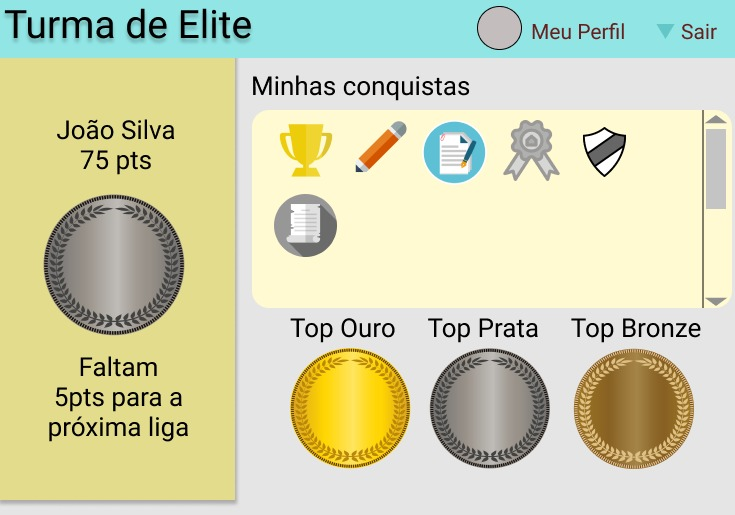
\includegraphics[width=11cm]{imagens/tela-aluno-2.jpeg}
	\caption{\textit{\gls{wireframe}} da tela do aluno}
	\fonte{Os autores}
\end{figure}
\FloatBarrier

\item \textbf{Perfil professor}: poderá visualizar as turmas atribuídas a ele e o ranking da turma. Será responsável por postar as atividades e ao corrigi-las, atribuir a pontuação para os alunos. A Figura 4 exibe um \textit{\gls{wireframe}} da tela para o perfil do professor.

\begin{figure}[htb]
    \centering
	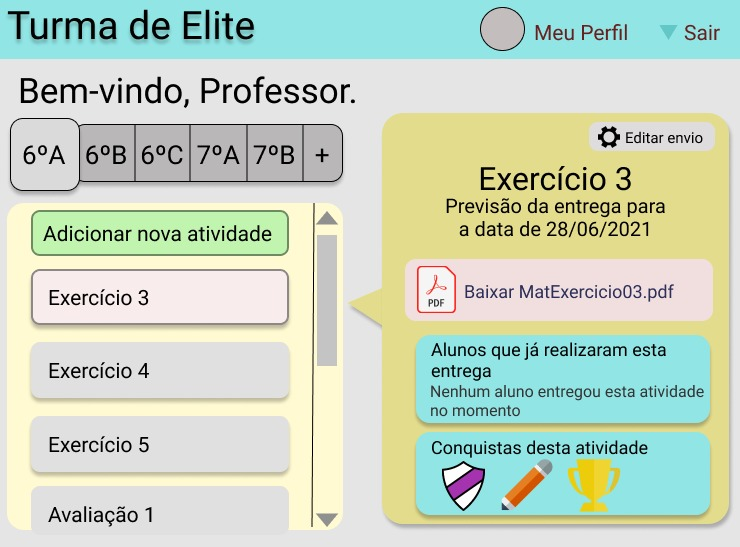
\includegraphics[width=11cm]{imagens/tela-professor.jpeg}
	\caption{\textit{\gls{wireframe}} da tela do professor}
	\fonte{Os autores}
\end{figure}
\FloatBarrier

\item \textbf{Perfil gestor}: poderá visualizar todas as turmas cadastradas, o ranking de cada uma delas e o \textit{\gls{dashboard}}. Será responsável por realizar os cadastros e parametrizações do sistema. A Figura 5 exibe um \textit{\gls{wireframe}} da tela para o perfil do gestor.

\begin{figure}[htb]
    \centering
	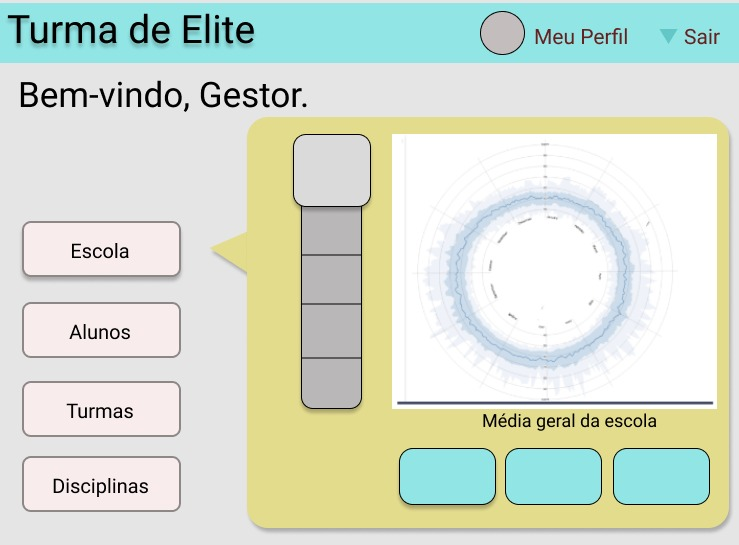
\includegraphics[width=11cm]{imagens/tela-gestor.jpeg}
	\caption{\textit{\gls{wireframe}} da tela do gestor}
	\fonte{Os autores}
\end{figure}
\FloatBarrier

\item \textbf{Perfil administrador}: Superusuário do sistema, será responsável pelo cadastro das escolas e seus respectivos gestores.
\end{itemize}


\subsection{Cadastros/Dados mestres}
Segundo os objetivos do projeto, são listados abaixo os cadastros básicos, essenciais ao funcionamento do sistema em questão. Para cada cadastro, o sistema deve permitir a inserção, listagem, alteração e exclusão (ou inativação) de registros. 
\begin{itemize}
\item \textbf{Usuários}: contempla os dados dos usuários que acessarão o sistema (gestores, professores e alunos).
\item \textbf{Turmas/disciplinas}: contempla os dados das turmas/disciplinas da escola;
\item \textbf{Conquistas}: contempla os dados das conquistas. Ao cadastrar uma conquista, o gestor deverá definir a recompensa pela sua conquista, o seu nível e os critérios para alcançá-la.
\item \textbf{Atividades}: contempla os dados das atividades. Uma atividade poderá gerar um entregável ou não.
\item \textbf{Escolas}: contempla os dados das escolas clientes da aplicação.
\end{itemize}


\subsection{Parametrização de turmas}
O gestor deverá utilizar esta funcionalidade para atribuir a cada turma, o professor responsável e os alunos. Para cada turma poderá ser atribuído um único professor. No caso de uma disciplina compartilhar mais de um professor, o gestor deverá criar uma disciplina para a mesma turma para cada professor e dividir os alunos entre elas. 

\subsection{Painel de turmas/disciplinas}
Este painel será exibido assim que o usuário acessar aplicação. Ele consiste em uma grade de botões que darão acesso ao ambiente da disciplina. Este painel estará disponível para as três visões previstas neste projeto, porém as turmas a serem listadas serão restringidas da seguinte forma:

\begin{itemize}
\item \textbf{Visão do aluno}: listará somente as disciplinas da turma no qual foi inserido.
\item \textbf{Visão do professor}: listará somente as turmas/disciplinas atribuídas a ele.
\item \textbf{Visão do gestor}: listará todas as turmas/disciplinas cadastradas.
\end{itemize}


\subsection{Módulo de atividades}
Este módulo será disponibilizado no ambiente da disciplina e será utilizado por professores e alunos. Através dele, o professor poderá postar as atividades e atribuir notas. Ao postar uma atividade o professor poderá informar a pontuação e o prazo de entrega. Caso a atividade possua um entregável, o professor deverá indicar também no momento do cadastro.


Para os alunos, ao acessar esta seção, eles poderão visualizar as atividades postadas pelo professor. Ao realizar uma atividade que necessita de um entregável, o aluno deverá realizar o \textit{upload} de um arquivo no formato especificado pelo professor na descrição da atividade, após a confirmação da entrega atividade ganhará um status “Pendente de avaliação”. Somente após a avaliação do professor, a atividade será marcada como concluída.


As atividades criadas que não geram entregáveis estão ligadas ao ensino presencial, na qual, ao passar uma atividade na sala, ou um dever de casa, o aluno mostrará a apostila para o professor, e ele dará o seu “visto” pela aplicação. 

\subsection{Painel de conquistas}
O painel de conquista estará disponível para o aluno. Cada aluno terá seu próprio painel de conquistas, e nele o aluno poderá visualizar as conquistas atingidas, as pendentes e as bloqueadas. 


O aluno poderá alcançar somente as conquistas atreladas a liga que ele se encontra e as imediatamente abaixo. A cada liga, as conquistas ficam mais difíceis de alcançar, porém as recompensas serão maiores. 
\subsection{Ranking de alunos por liga}
O sistema de ranqueamento do sistema Turma de Elite contemplará três ligas, sendo elas: bronze, prata e ouro. Cada liga conterá um ranking disponibilizado em duas visões (\textit{\gls{ranking}} por disciplina e \textit{\gls{ranking}} geral). Sempre ao final de um período pré-determinado, os três primeiros colocados de um ranking que possuem a pontuação mínima requerida pela liga superior, ganham um lugar na próxima liga, enquanto os três últimos descem para uma liga inferior.


Assim como o painel de turmas/disciplina, os \textit{\glspl{ranking}} estarão disponíveis para todos os usuários, porém de forma restringida dependendo do perfil.
\begin{itemize}
\item \textbf{Visão do aluno}: visualizará apenas os \glspl{ranking} referente à turma no qual o aluno está inserido. Em cada ranking o aluno saberá apenas o nome dos três primeiros colocados de cada liga e a sua posição caso ele não esteja entre os primeiros.
\item \textbf{Visão do professor}: visualizará os \glspl{ranking} das turmas atribuídas a ele. Em cada ranking, o professor poderá ver todos os alunos e suas respectivas posições.
\item \textbf{Visão do gestor}: visualizará os rankings de todas as turmas ativas na aplicação. Em cada \gls{ranking}, o gestor poderá ver todos os alunos e suas respectivas posições.
\end{itemize}

\subsection{Dashboard}
A aplicação também disponibilizará relatórios gerenciais para o perfil gestor como: histórico de desempenho por turma e por aluno.

%\section{Entrega Final}

%\itemPara a entrega completa do sistema Turma de Elite já está previsto, além de melhorias, %desenvolvimento de novas funcionalidades que %serão elencadas nos tópicos a seguir:
%\begin{itemize}
%\item  Criação do novo perfil "Pais e %responsáveis": melhoria no módulo de acesso, %o novo perfil permitirá que os pais ou %responsáveis pelo aluno acompanhe as %atividades do aluno.
%\item  Boletins: nova funcionalidade que %permitirá que os professores insiram as notas %das provas ao fim de cada bimestre.
%\item  Plano de aulas: nova funcionalidade %que permitirá que o professor realize seu %planejamento de aulas. Este plano de aulas %poderá ser convertido para um relatório que %estará disponível para download para os %gestores da escola;
%\item  Atividades programadas: melhoria que %permitirá que os professores programem a %postagem de atividades para seus alunos.
%\item  Notificações e Lembretes: melhoria que %permitirá que os usuários sejam notificados %por e-mail a respeito de ações tomadas na %aplicação como, por exemplo, confirmação de %envio de atividade.
%\end{itemize}



\section{\textit{Product Backlog}}
Com as histórias de usuário definidas, foi montado o \textit{Product Backlog} para definir a ordem de importância delas. A Figura 6 representa o resultado da priorização, segundo cada funcionalidade.  

\begin{figure}[htb]
    \centering
	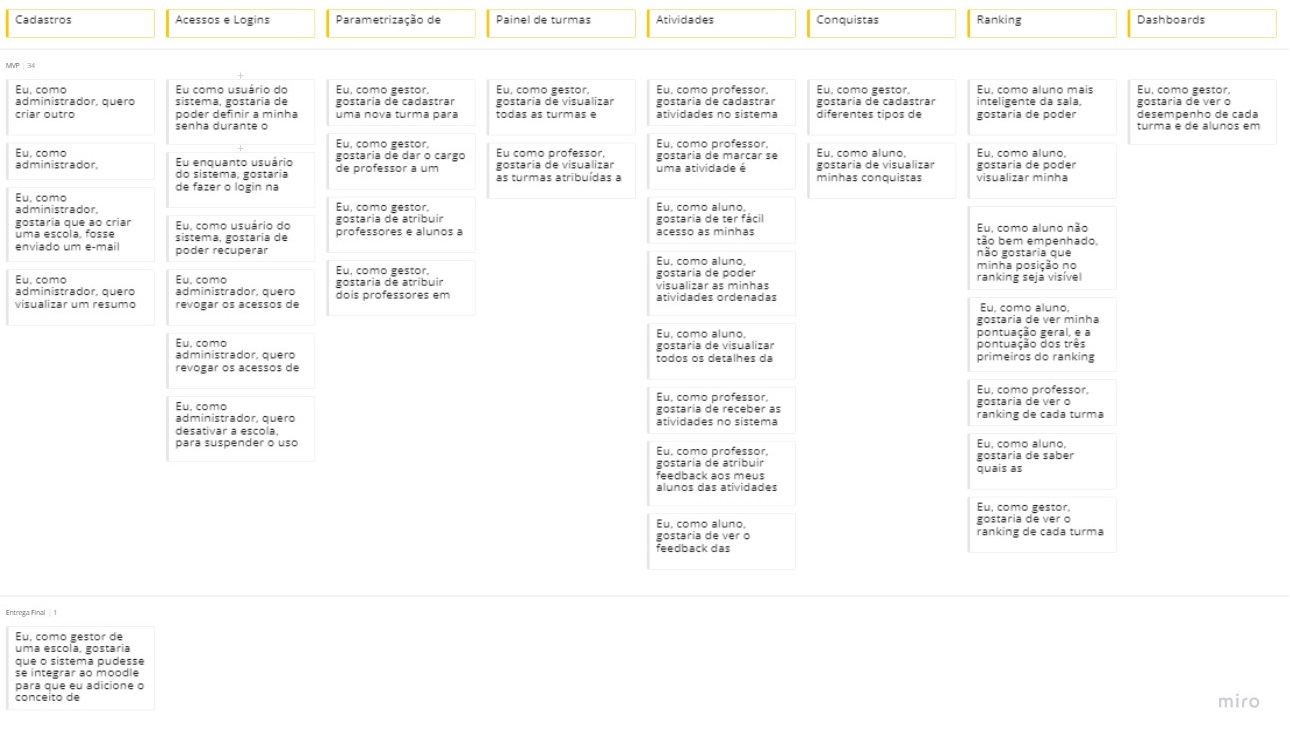
\includegraphics[width=16cm]{imagens/ProductBacklog.jpg}
	\caption{Product Backlog do Projeto Turma de Elite}
	\fonte{Os autores}
\end{figure}
\FloatBarrier

\section{MER e DER}
Para a modelagem de dados do projeto, foi elaborado o modelo entidade-relacionamento (MER) e, para representá-lo, foi feito o diagrama entidade-relacionamento (DER), conforme demostra a Figura 7.

\begin{figure}[htb]
    \centering
	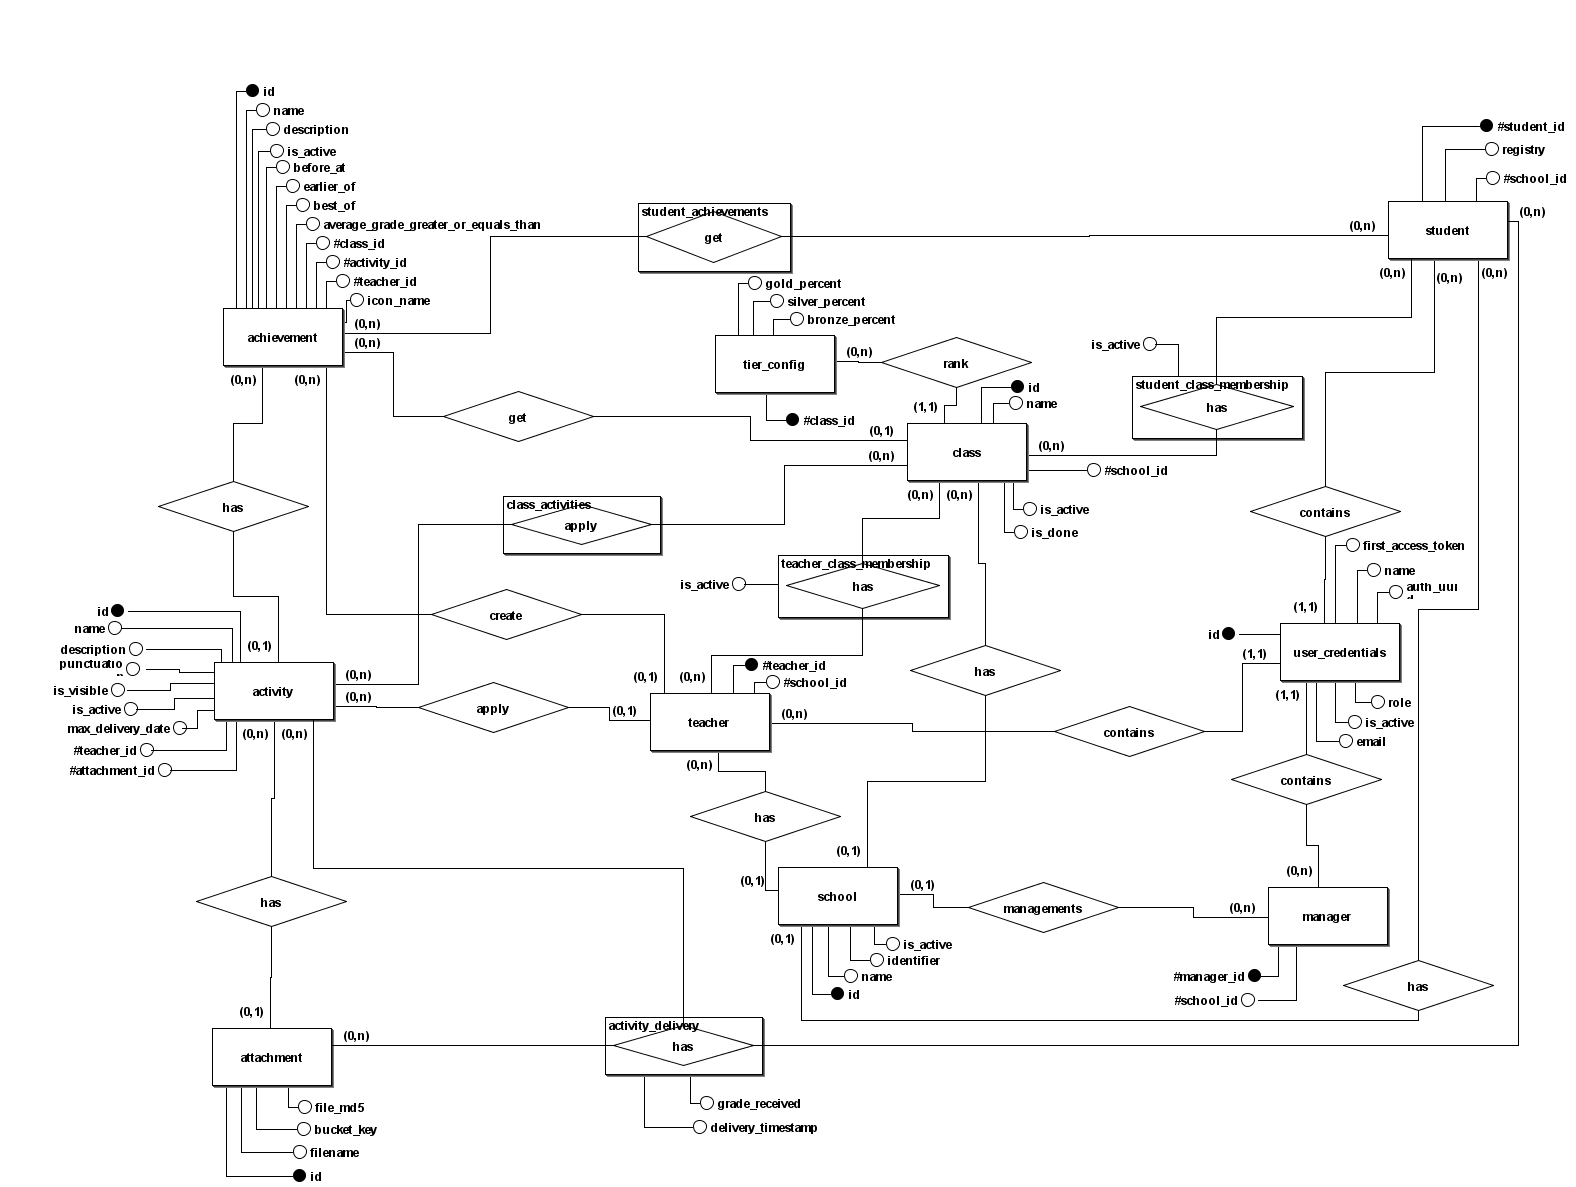
\includegraphics[width=16cm]{imagens/ModeloConceitual.png}
	\caption{Modelo Conceitual do Projeto Turma de Elite}
	\fonte{Os autores}
\end{figure}
\FloatBarrier


\section{Modelo Lógico}
Com o MER e DER mapeados, foi possível desenvolver o modelo lógico da aplicação, conforme mostra a figura 8.

\begin{figure}[htb]
    \centering
	\includegraphics[width=16cm]{imagens/ModeloLogico.png}
	\caption{Modelo Lógico do Projeto Turma de Elite}
	\fonte{Os autores}
\end{figure}
\FloatBarrier

\chapter{Viabilidade financeira}
O fato da aplicação ser \textit{\gls{open-source}} restringe a possibilidade de se ganhar dinheiro com venda direta, porém possibilita obtenção de lucro por meio de outras formas, como por exemplo:

\begin{itemize}
   \item \textbf{Utilização do servidor do fornecedor}: Nessa ocasião, a empresa contratante pagará um aluguel mensal para utilizar a aplicação hospedada no servidor do fornecedor.
   \item \textbf{Utilização de servidor próprio}: Utilização da aplicação em um servidor próprio da empresa contratante via pagamento de uma taxa de implementação mais uma de manutenção. Apesar de pagar mais pela implementação em um servidor próprio, a empresa contratante terá o direito de personalizar o produto de acordo com suas preferências nesse método de cobrança.
\end{itemize}

Há ainda a possibilidade de compilação independente do código-fonte da aplicação, por conta da premissa \textit{\gls{open-source}} citada anteriormente. Nesses casos, o fornecedor não se responsabilizará pela prestação de suporte.


Como forma de manter a aplicação, será cobrada uma taxa de R\$10,00 de cada aluno (sendo pago por ele ou pelo mantenedor da instituição de ensino) para que seu acesso à aplicação seja concedido. Desse modo, os custos com hospedagem já estariam cobertos a longo prazo. A Tabela 4 exibe uma previsão orçamentária para o projeto.

\ABNTEXfontereduzida
\begin{table}[htb]
\centering
\caption{Previsão orçamentária mensal do Projeto Turma de Elite}
\begin{tabular}{|p{2.5cm}|c|c|c|c|c|}
   \hline
   \thead{} & \thead{100 alunos}  & \thead{1000 alunos}  & \thead{5000 alunos} & \thead{10000 alunos} & \thead{50000 alunos} \\\hline
   Heroku & R\$127* & R\$506* & R\$1010* & R\$5048* & R\$10096*  \\\hline
    Firebase Hosting & R\$0 & R\$177* & R\$411* & R\$832* & R\$5689* \\\hline
    Firebase Authentication & R\$0 & R\$0 & R\$0 & R\$3029* & R\$18172* \\\hline
    Receita & R\$1000 & R\$10000 & R\$50000 & R\$100000 & R\$500000 \\\hline
    Lucro & R\$873 & R\$9317 & R\$48579 & R\$91091 & R\$466043\\\hline
\end{tabular}
\fonte{Dados do Projeto}
\legend{* - O valor exibido foi aproximado com base na cotação do dólar americano para o dia 08/06/2021 (US\$1 = R\$5,04)}
\end{table}

Com relação aos \textit{\gls{dyno}} do \textit{Heroku} para hospedar a quantidade crescente de acessos concorrentes, a relação obtida foi:
\begin{itemize}
    \item \textbf{100 alunos}: 1 \textit{\gls{dyno}} - \textit{Standard} 1X
    \item \textbf{1000 alunos}: 2 \textit{\glspl{dyno}} - Standard 2X
    \item \textbf{5000 alunos}: 4 \textit{\glspl{dyno}} - Standard 2X
    \item \textbf{10000 alunos}: 4 \textit{\glspl{dyno}} - Performance M
    \item \textbf{50000 alunos}: 2 \textit{\glspl{dyno}} - Performance L
\end{itemize}

A Figura 7 apresenta as relações de preço presentes no website do Heroku.

\begin{figure}[htb]
    \centering
	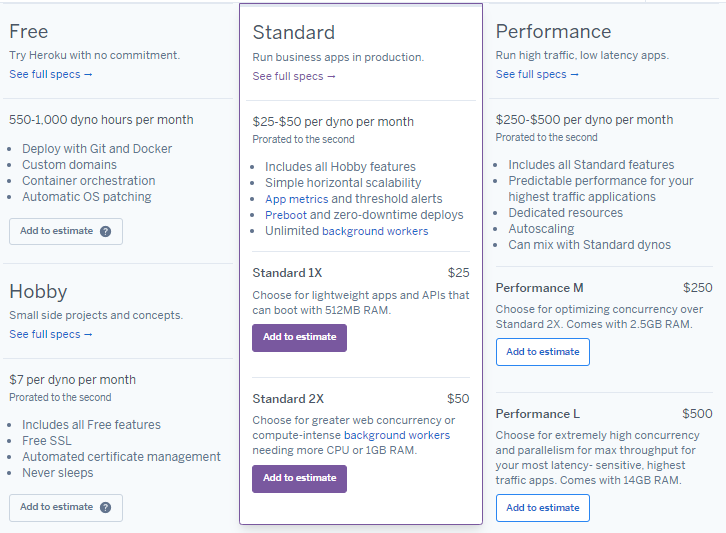
\includegraphics[width=16cm]{imagens/precos-heroku.png}
	\caption{Preço mensal de aluguel dos \textit{\glspl{dyno}} do Heroku}
	\fonte{\cite{heroku:2021}}
\end{figure}


O custo de hospedagem e autenticação variou conforme a quantidade de armazenamento e suporte a acessos simultâneos necessários para atender a quantidade crescente de alunos.

% ----------------------------------------------------------
% Finaliza a parte no bookmark do PDF
% para que se inicie o bookmark na raiz
% e adiciona espaço de parte no Sumário
% ----------------------------------------------------------
\phantompart

% ----------------------------------------------------------
% Referências bibliográficas
% ----------------------------------------------------------
% quando não esta utilizando biblatex tem que carregar as referencias aqui
\IfPackageLoaded{biblatex}{}{%
\bibliography{referencias,exemplos/abntex2-doc-abnt-6023}
}

% ----------------------------------------------------------
% Glossário
% ----------------------------------------------------------
%

 \ifdef{\printnoidxglossary}{
     \addcontentsline{toc}{chapter}{GLOSSÁRIO}
     \printnoidxglossary[style=glossario]
}{}

\end{document}